\chapter{Auswahl der Komponenten}
Die Auswahl der Komponenten hängt maßgäblich von den Anforderungen und den lokalen gegebenheiten ab.


\section{Motoransteuerung}

\usnsection{Treiberbausteine}
Da die gewählten Akkus eine Spannung von 14,4V aufweisen, kann der orgiginal Motortreib erleider nicht verwendet werden.
Denn dieser benötig eine Spannung von 7,4V. Da der AVR Mikrokontroller mit 5V betrieben wird, wird ein Motorteiber benötig der
mit den 5V Pegeln arbeiten kann. In vielen Mikrocontroller Projekten und in unserem ersten Prototyp wird der L298 DUAL FULL-BRIDGE DRIVER
verwendet. Dieser ist leider auch bei der Benutzung beider Kanäle auf 4 Ampere begrenzt \cite{L298}, was beim Prototy zu einer Permanenten
überlastung des Treibers führt. Leider sind keine vollintegrierten Motortreiber mit der benötigten Belastbarkeit verfügbar.
Um die bentötigte Belastbarkeit zu erreichen wird der zur Ansteuerung benötigte Vierquadrantensteller aus diskreten Mosfets aufgebaut.

\subsubsection{Vierquadrantensteller}
Definition nach Wikipedia:\\
``Ein Vierquadrantensteller besteht aus einer elektronischen H-Brückenschaltung aus vier Halbleiterschaltern, meist aus Transistoren, 
welche eine Gleichspannung in eine Wechselspannung variabler Frequenz und variabler Pulsbreite umwandeln kann. Vierquadrantensteller 
in der Energietechnik können auch Wechselspannungen unterschiedlicher Frequenzen in beiden Richtungen ineinander umwandeln.''


\begin{figure}[H]
\centering
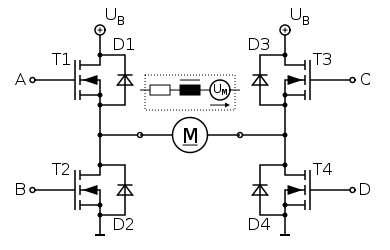
\includegraphics[width=.8\textwidth]{Vierquadrantensteller.png}\\
\caption{Vierquadrantensteller}%
\label{fig:Vierquadrantensteller}
\end{figure}


Auf Grund der hohen Belastbarkeit werden meißt Mosfets als Halbleiterschalter genutzt. Um die beiden oberen Mosfets (T1/T3) durchzuschalten
ist auf Grund des fehlenden Massepotentials eine Gatespannung oberhalb der Betriebsspannung nötig. Diese wird meist mittels Bootstrapping zur
Verfügung gestellt. Da das simultane Durchschalten der Übereinander liegenden Mosfets zu einem Kurzschluss führen würde, muss dies durch
eine Schutzschalung verhindert werden. Um all diese Funktionen zur verfügung zu stellen gibt es bereits fertige Mosfettreiber,
was das Schaltungsdesign enorm vereinfacht.

\subsection{Mosfettreiber}
\subsubsection{Verfügbarkeit}

Mosfettreiber gint es in vielenAusführungen, unter anderem als ``Single Channel High Side Driver``, ``Half Bridge Driver'', ``Full Bridge Driver''
und ``3 Phase Driver''. Da für den Verbauten DC-Motor eine Vollbrücke nötig ist, um den Motro in alle Richtungen zu betreiben, Werden an dieser Stelle
ausschließlich ``Full Bridge Driver'' untersucht.

Eine Tabelle auf Mikrocontroller.net\cite{FET_D_TABLE} zeigt eine Auswahl an verfügbaren Mosfettreibern. Dort sind zwei
``Full Bridge Driver'' aufgeführt, welche für dieses Projekt passend sind. Allerdings fällt die Entscheidung auf einen anderen Treiber,
dem Allegro A3941.
\subsubsection{Allegro A3941}
Der Allegro A3941 ist f+r Betriebsspannungen von 5,5V bis 50V geeignet und liegt damit in der Spezifikation des Projekts.
Des weiteren verfügt der Motor über eine integrierten 5V Regulator und kann somit ohne Spannungsregulator am Akku betrieben werden.
Über zwei Ausgänge der Treibers können diverse Fehler ausgelesen werden.


Der Treiber lässt sich in verscjiedennenModi betreiben:

\begin{figure}[H]
\centering
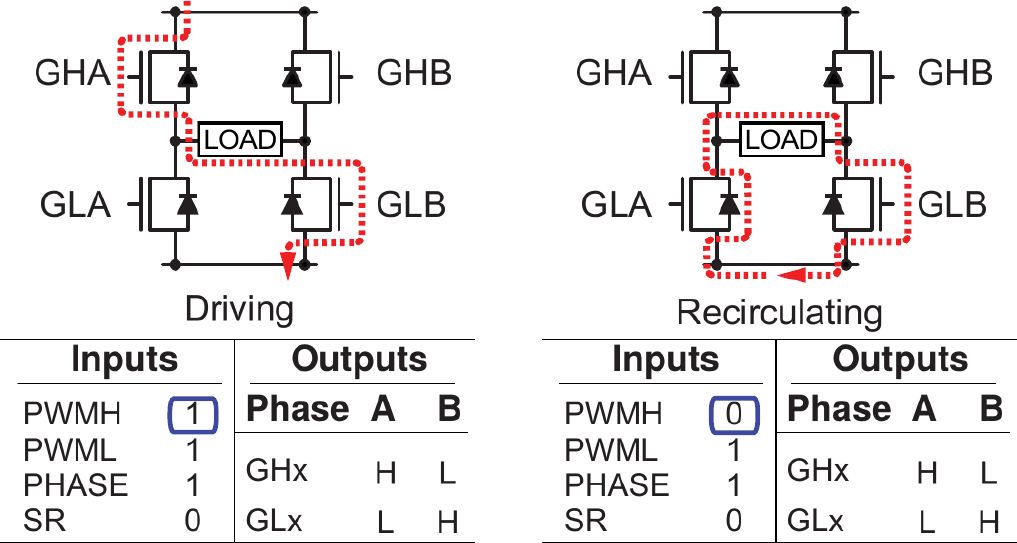
\includegraphics[width=.8\textwidth]{3941_1.png}\\
\caption{Slow decay, diode recirculation, high-side PWM}%
\label{fig:3941_1}
\end{figure}

Konfiguration: PWML=1, PHASE=1, SR=0 und PWM an PWMH (high-side PWM)\\
Bei aktivierten PWMH fließt der Strom durch den GHA-Mosfets über den Motor und
dann über den GLB-Mosfet. in diesem Modus wird der Motor angetrieben.
Wenn PWML deaktiviert ist zirkuliert der vom Motor induziert Strom durch GLB und durch
die interne Diode von GLA, der Motor wird dadurch gebremst.


\begin{figure}[H]
\centering
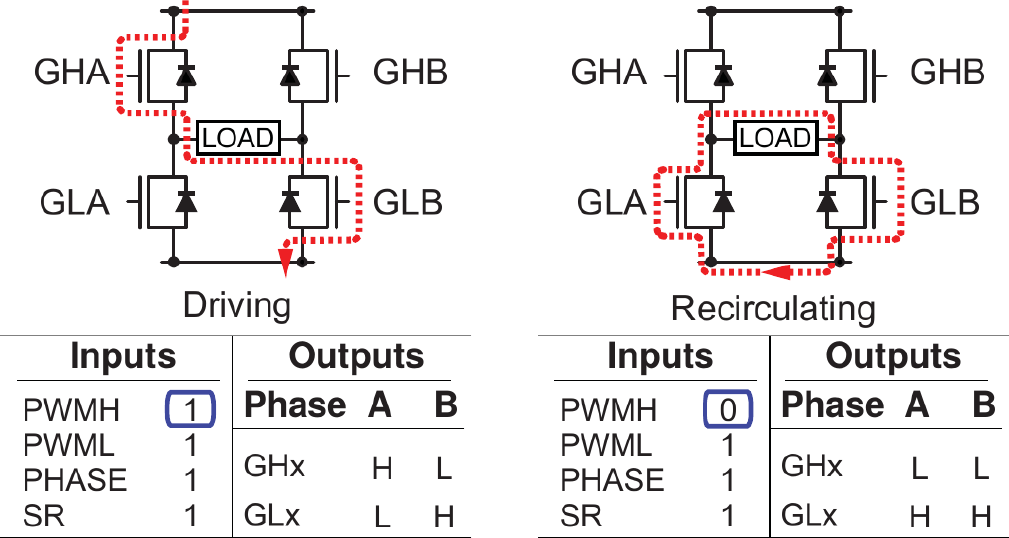
\includegraphics[width=.8\textwidth]{3941_2.png}\\
\caption{Slow decay, SR active, high-side PWM}%
\label{fig:3941_2}
\end{figure}

Konfiguration: PWML=1, PHASE=1, SR=1 und PWM an PWMH (high-side PWM)\\
Bei aktivierten PWMH fließt der Strom durch den GHA-Mosfets über den Motor und
dann über den GLB-Mosfet. in diesem Modus wird der Motor angetrieben.
Wenn PWML deaktiviert ist zirkuliert der vom Motor induziert Strom durch 
GLB und durch GLA, der Motor wird durch den niedrigeren Innenwiederstand des Mosfest 
stärker gebremst als in der Voherigen Konfiguration. Dabei ist darauf zu achten, dass
beinahe die gesamte induzierte Spannung über den beiden Mosfets (GLA/GLB) abfällt.
Was zu einer starken Hitzeentwicklung führen kann.



\begin{figure}[H]
\centering
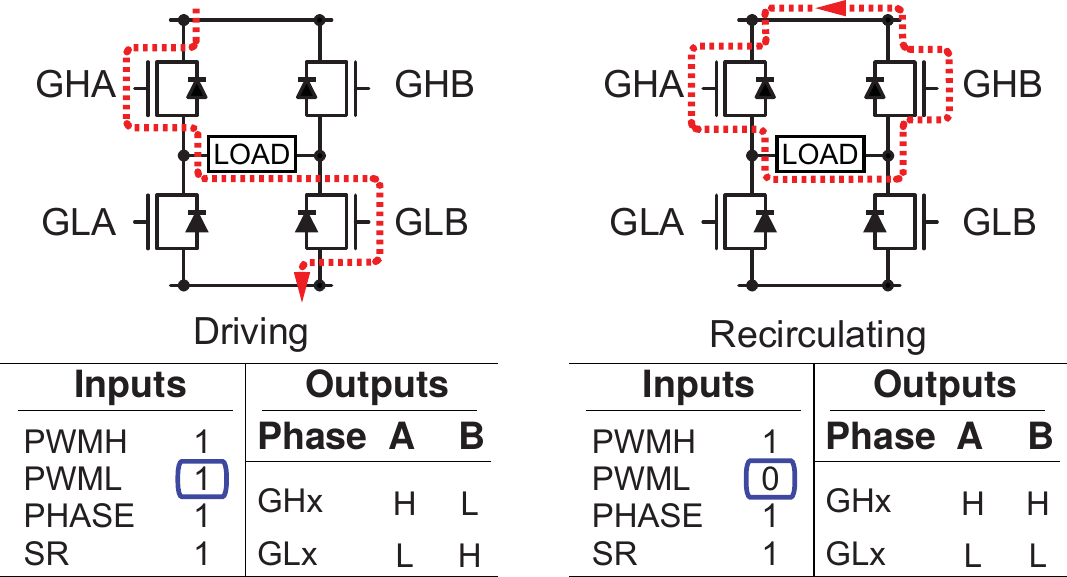
\includegraphics[width=.8\textwidth]{3941_3.png}\\
\caption{Slow decay, SR active, low-side PWM}%
\label{fig:3941_3}
\end{figure}

Konfiguration: PWMH=1, PHASE=1, SR=1 und PWM an PWML (low-side PWM)\\
Diese Konfiguration entspricht im Grunde den beiden vorherigen, Nur das dass PWM-Signal
an den unteren Mosfets anliegt. Der SR-Pin entscheidet wieder darüber ob im ``Bremsmodus''
die internen Dioden genutzt werden (SR=0) oder nicht (SR=1)




\begin{figure}[H]
\centering
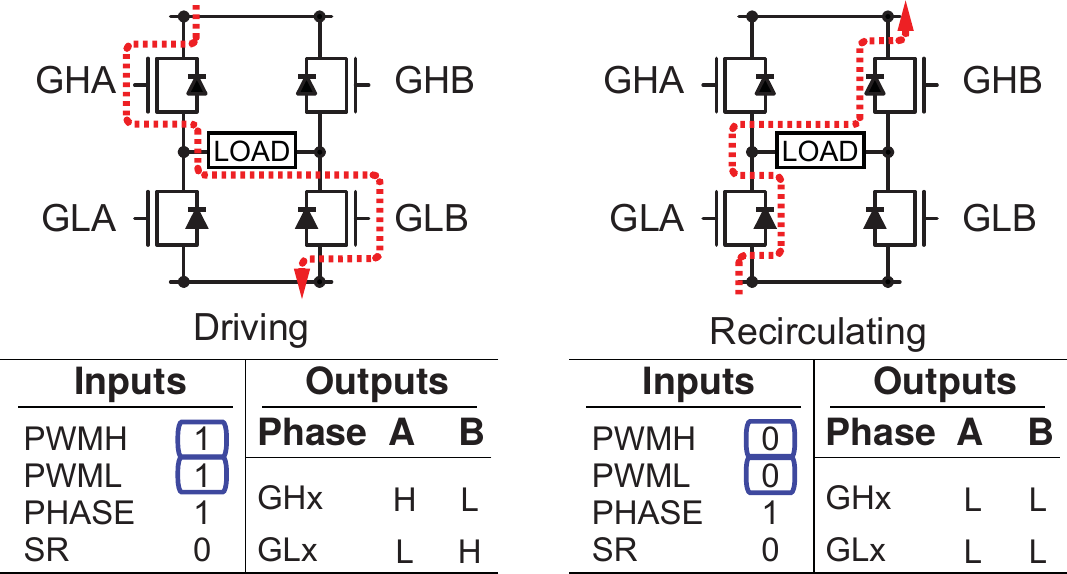
\includegraphics[width=.8\textwidth]{3941_4.png}\\
\caption{Fast decay, diode recirculation}%
\label{fig:3941_4}
\end{figure}


Konfiguration: PWMH=1, PWML=1, PHASE=1, SR=1\\
in dieser Konfiguration werden die oberen und unteren Mosfets gleich geschaltet. Im
``Bremsmodus'' führt das dazu das der induzierte Motorstrom nicht über die Mosfets
zirkulieren kann. Der Strom fließt stattdessen zurück in die Spannungsquelle, was
abhängig von der Spannungsquelle zu Schäden führen kann. Wird die Schaltung jedoch an
einem Akku betrieben ist es so möglich die Energie zu nutzen und damit den Akku
zu laden.

\begin{figure}[H]
\centering
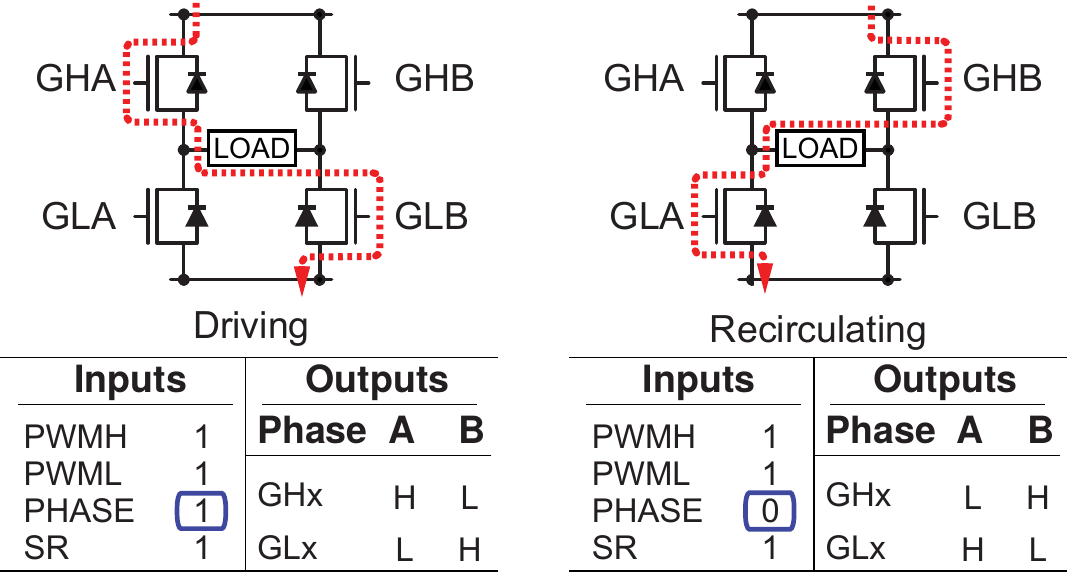
\includegraphics[width=.8\textwidth]{3941_5.png}\\
\caption{Fast decay, SR active, full four-quadrant control}%
\label{fig:3941_5}
\end{figure}

Diese Konfiguration zeigt den Einfluss des PHASE-Pins. Liegt am PHASE-Pin 1 ein an
fließt der Strom von links nach rechts. Liegt 0 an fließt er von rechts nach links.
Mithilfe des PHASE-Pins wird also die Polung des Motors festgelegt.


